\documentclass{asaproc}

\usepackage{amsmath}
\usepackage{float}
%\usepackage{times}
%If you have times installed on your system, please
%uncomment the line above

\usepackage{natbib}
\usepackage[export]{adjustbox}

\newtheorem{defn}{Definition}
%For figures and tables to stretch across two columns
%use \begin{figure*} \end{figure*} and
%\begin{table*}\end{table*}
% please place figures & tables as close as possible
% to text references
\usepackage{graphicx}

\newcommand{\Capyi}{Y_i}
\newcommand{\Yequalsy}{\Capyi = \yi}
\newcommand{\lcni}{n_i}
\newcommand{\sumyiO}{\sum_{\lcni = 0} ^ \infty}
\newcommand{\sumyiNi}{\sum_{\lcni=\yi} ^ \infty}

\newcommand{\prodi}{\prod_{i=1}^n}
\newcommand{\yi}{y_i}
\newcommand{\sumi}{\sum_{i=1}^n}
\newcommand{\squarebk}[1]{\left[#1\right]}
\newcommand{\parenth}[1]{\left(#1\right)}
\newcommand{\curlies}[1]{ \left\{#1\right\} }
\newcommand\tab[1][1cm]{\hspace*{#1}}
\newcommand{\Pois}{\text{Pois}}
\newcommand{\Gam}{\text{Gamma}}
\newcommand{\Bin}{\text{Bin}}
\newcommand{\be}{\begin{equation}}
\newcommand{\ee}{\end{equation}}
 \title{Red Hawk Sightings in California}
\newcommand{\alplam}{\alpha_\lambda}
\newcommand{\betlam}{\beta_\lambda}
\newcommand{\betthet}{\beta_\theta}
\newcommand{\lami}{\lambda_i}
\newcommand{\theti}{\theta_i}
\newcommand{\ci}{c_i}
\newcommand{\Ni}{N_i}
\newcommand{\Bet}{\text{Beta}}
%input all authors' names

\author{Mary Silva\\
AMS 207 - Take Home Exam 1}

%input affiliations

%{USDA Forest Service Forest Products Laboratory}

\begin{document}

\maketitle

%\begin{figure}[h]
%    \includegraphics[width=0.5\textwidth]{Rplot05.pdf}
%    \caption{Airport locations}
%    \label{fig:loc}
%\end{figure}




\begin{abstract}
The North American Breeding survey provides information about the abundance of different species of birds in North America. We look to examine the counts of Red Hawk sightings in California using a Bayesian Hierarchical model.
\begin{keywords}
Hierarchical model, rejection sampling, Poisson-Gamma model, North American Breeding Survey.
\end{keywords}
\end{abstract}

\begin{table}[ht]
\centering
\caption{A portion of the data from North American Breeding Survery for the years 1968 - 1977 showing the counts of Red-tailed Hawks in California and the Route Counts for each year.}
\label{BirdDat}
\begin{tabular}{rrrr}\\\\
  \hline
 & years & Route Count & Red-tailed Hawk \\ 
  \hline
1 & 1968 &  26 &  73 \\ 
  2 & 1969 &  31 &  81 \\ 
  3 & 1970 &  59 & 157 \\ 
  4 & 1971 &  59 & 131 \\ 
  5 & 1972 & 128 & 307 \\ 
  6 & 1973 & 151 & 284 \\ 
  7 & 1974 & 145 & 364 \\ 
  8 & 1975 & 150 & 381 \\ 
  9 & 1976 & 144 & 405 \\ 
  10 & 1977 & 144 & 367 \\ 
   \hline
\end{tabular}

\end{table}



\section{Introduction}
The data is obtained from the North American Breeding Survey for Red Hawks in California (Table \ref{BirdDat}). The full data set contains the years 1977 through 2017. The variables of interest are the bird route counts and the counts of Red Hawk sightings.

Initial exploratory analysis shows an increasing trend of Red Hawk sightings over time (Figure \ref{scatter_Eda}) as well as an increasing trend in bird flight route counts (Figure \ref{Routes}). We see that the density for red hawk sightings in California \ref{HistDensOriginal} is multimodal and skewed, which should be taken into consideration when building a model.

\begin{figure}
    \centering
    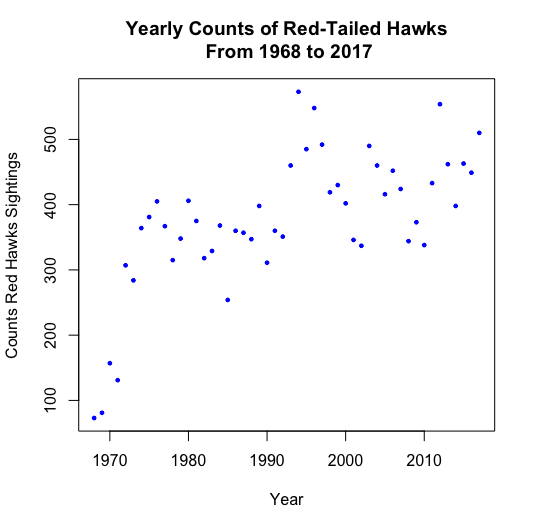
\includegraphics[scale=0.4]{Scatter_EDA.png}
    \caption{Scatter plot of the counts of Red Hawk Sightings by year in California}
    \label{scatter_Eda}
\end{figure}

\begin{figure}
    \centering
    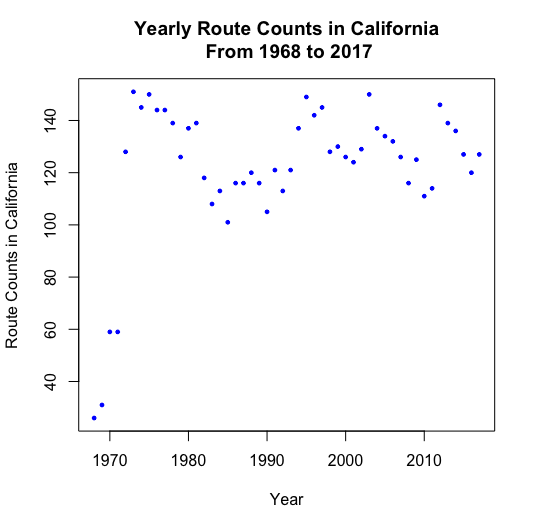
\includegraphics[scale=0.4]{Routes.png}
    \caption{Scatter plot of the route counts for California over time}
    \label{Routes}
\end{figure}
\begin{figure}
    \centering
    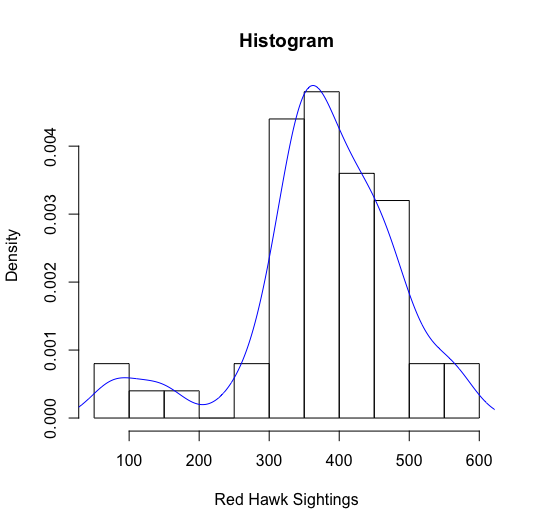
\includegraphics[scale=0.35]{Hist_Dens.png}
    \caption{A histogram plot of the Red Hawk sightings in California with a density overlay}
    \label{HistDensOriginal}
\end{figure}

\section{Model 1}
\textbf{Note that I have modified Model 1 from my original takehome as you suggested.} Given that we are dealing with count data, it is reasonable to consider the red hawk sightings $(y_i)$ to be distributed from a Beta-Binomial model, or as Poisson-Gamma model. 

\subsection{M1: Specifications}
Model 1 now incorporates the rate counts appropriately and I used a simpler hierarchical structure as follows
\begin{align*}
    y_i &\sim \Pois(\lambda_i c_i)\\
    \lambda_i &\sim \text{Exp}(\theta)\\
    \theta &\sim \Gam(\alpha, \beta) 
\end{align*}
Where the values $\alpha$ and $\beta$ are fixed. The joint posterior distribution for the above mentioned model then becomes
\begin{align*}
    p(\lambda, \theta | y) &\propto \prodi \left[ f(y|\lambda_i, c_i) \pi(\lambda_i|\theta) \right]\pi(\theta)\\
    &\propto \prodi \left[ \frac{(c_i \lambda_i)^{y_i} \exp\left\{-\lambda_i c_i \right\} }{y_i!} \theta \exp\left\{-\theta \lambda_i \right\} \right]\\
    & \tab\times \frac{\beta^\alpha}{\Gamma(\alpha)} \theta^{\alpha -1 }\exp\left\{-\beta\theta \right\}
\end{align*}

The full conditionals (up to proportionality) under this model specification are as follows
\begin{align*}
    \lambda_i\Big|\cdot &\sim \Gam\Big(\lambda_i \Big|y_i + 1, c_i + \theta\Big)\\
    \theta\Big|\cdot &\sim \Gam\left(\theta \Big|n + \alpha, \beta + \sumi \lambda_i \right)
\end{align*}

Since the full conditionals (under this model specification) are known distributions, I re-implemented model 1 using a straightforward Gibbs sampling approach. 

\section{Model 2}
\subsection{Specifications}
Next, we will consider a modification of model 1 as follows
\begin{align*}
    y_i &\sim \Bin(N_i,\theta_i)\\
    N_i &\sim \Pois(\lambda_i c_i)\\
    \lambda_i &\sim \Gam(\alplam,\betlam)\\
    \theta_i &\sim \Bet(1, \betlam)
\end{align*}

where $y_i$ corresponds to the observed count of hawks, out of a population of $N_i$ hawks for the $i^\text{th}$ year. Unfortunately, $N_i$ is not known, so we assign a discrete prior. 

The joint posterior is given by the following
\begin{align*}
    p(\Ni, \theti, \lami| y) \propto& \prodi \Big[ f(y_i|\Ni,\theti) \pi(\Ni|\lami, \ci)\Big]\\
    & \tab \times \prodi \Big[ \pi(\lami|\alplam, \betlam) \pi(\theti|\betthet) \Big]\\
    \propto& \prodi \left[ \frac{\betlam^{\alplam}}{\Gamma(\alplam)} \frac{1}{Be(1,\betlam)} \frac{1}{y_i! (\Ni - y_i)!} \right]\\
    &\times \prodi \left[ \lami^{\Ni + \alplam - 1} \exp\left\{-\lami(\ci + \betlam) \right\} \right]\\
    &\times \prodi \squarebk{\ci^{\Ni} \theti^{y_i}(1-\theti)^{\Ni - \yi + \betthet-1}}
\end{align*}
The conditionals under this model specification (up to proportionality) are as follows
\begin{align*}
    &\theti | \cdot \sim \Bet \parenth{\theti\Big| \yi + 1, \Ni - \yi +\betthet}\\
    &\lami|\cdot \sim \Gam\parenth{\lami \Big| \Ni + \alplam, \ci + \betlam}\\
    &\pi_N(\Ni|\cdot) \propto \frac{1}{(\Ni - \yi)!} (\ci\lami)^{\Ni}(1-\theti)^{Ni}
\end{align*}
The hyper parameters of the priors $\alplam, \betlam, \betthet$ are fixed, and the choice of hyperparameter will be described in the next section.

\subsection{M2: Sampling Algorithm}
The full conditional for $\Ni$ is not a recognizable distribution. So, unlike model 1, a Gibbs sampling algorithm is not appropriate. 

We consider a Metropolis-Hastings algorithm, in which we sample a proposed $\Ni^*$ from a proposal distribution at each iteration $t$. Since we know that $\Ni$ is the population of hawks, our \textit{proposal distribution must be discrete}. Ultimately, I decide to use a Poisson distribution as my proposal distribution for $\Ni^*$. We know that the proposal distribution should have a mean centered around the rate of the population of red-hawks, $\lami \ci$, so we use our $\lami$ samples at each iteration as a parameter for our proposal distribution. The $\ci$, of course, are fixed. We are unable to use a Metropolis-within-Gibbs sampling algorithm since that requires the proposal distribution to be symmetric. (I did also consider a Binomial proposal distribution, but in the short time frame I went with Poisson and didn't look back).

We use 20000 iterations with a burn-in of 2000. At each iteration we compute the following ratio

\begin{align*}
    r = \frac{\pi_N(\Ni^*|\lami, \theti, \cdot) / J(\Ni^*|N^{(t-1)}_{i})}{\pi_N(N^{(t-1)}_{i}|\lami, \theti,\cdot)/J(N^{(t-1)}_{i}|\Ni^*)}
\end{align*}

Where $J(\cdot|\cdot)$ is our proposal distribution. We then set

$$ \Ni^{(t)} = \begin{cases} 
      \Ni^* & \text{with probability $min(r,1)$}\\
      N^{(t-1)}_{i} & \text{otherwise.}
   \end{cases}
$$
which requires the generation of a uniform random number. Based on our hyperparameters and proposal density, we have an acceptance ratio that is approximately $80\%$. The ideal range is between 20-25\%, but autotuning our acceptance rate to a target hasn't really been discussed so I am not going to do this.

%I determine that either a Binomial distribution or a Poisson distribution are appropriate. Ultimately, I chose the Poisson distribution, since it relied only on the rate parameter. The Binomial on the other hand relies on two parameters: the number of trials and their corresponding probabilities (honestly two parameters sounded like more work and thought needed to be applied, I now realize that's not the case).

\subsection{M2: Hyperparameter Choice}
For this model, we do have some prior knowledge of the population $\Ni$ of hawks in the sense that we know this number should be large (there's 1.9 million red hawks in North America alone according to a quick google search). I used this prior knowledge as a starting point. In other words, we need $\lami\ci$ to be very high. Since $\ci$ is fixed, we can only control the $\lami$. 

Since $\lami$ is just a latent variable with no interpretation, we can choose any $\alplam$ and $\betlam$ such that $E(\lami)$ is large and $V(\lami)$ is small. This was a trial and error assessment, similar to homework 2. Ultimately, I decide to set $\alplam = 10000$ and $\betlam = 10$, which leads to $E(\lami) = \frac{\alplam}{\betlam} = 1000$ and $V(\lami) = \frac{\alplam}{\betlam^2} = 100$.

Next we look at the hyper parameter for $\theti$, $\betthet$. We have to ensure that our prior mean for theta, $E(\theta) = \frac{1}{1+\betthet}$, is proportional to the MLE, $ \text{mean}(\yi)/\Ni$. Thus, we select $\betthet = 500$. 

As one last sanity check, we can look at the mean of the data, $mean(\yi) = 376.1$ and compare it to the mean of the samples (i.e. $mean(N^{(1:iters)}_{i}\times\theta^{(1:iters)}_{i}) = 375.5692$). We see that these numbers are close, which means that our MCMC samples are converging to reasonable estimates. 

\subsection{M2: Parameter Inference}
To check for mixing and convergence we examine the sampling traces for the parameters. 

First we look at the population count $\Ni$. Based on the trace plots, histograms, and autocorrelation plots for randomly selected years (Figures \ref{traceN1} - \ref{traceN48}). We see that our M-H sampler is mixing and converging.  This autocorrelation is clearly decreasing as the lag increases (i.e. samples can be considered as independent). We summarize a few years in table \ref{Nisummary}. 


\begin{table}[h!]
\centering

\begin{tabular}{rrrr}
  \hline
 Year& Mean & 2.5\% & 97.5\% \\ 
  \hline
1968 & 26002.57 & 25493.00 & 25659.00 \\ 
  1982 & 118043.31 & 115969.95 & 116633.00 \\ 
  1998 & 127982.51 & 125774.95 & 126487.00 \\ 
  2015 & 127026.29 & 124794.00 & 125512.00 \\ 
   \hline
\end{tabular}
\caption{Summary of MCMC samples of population count by year.}
\label{Nisummary}
\end{table}


\begin{figure}[h!]
    \centering
    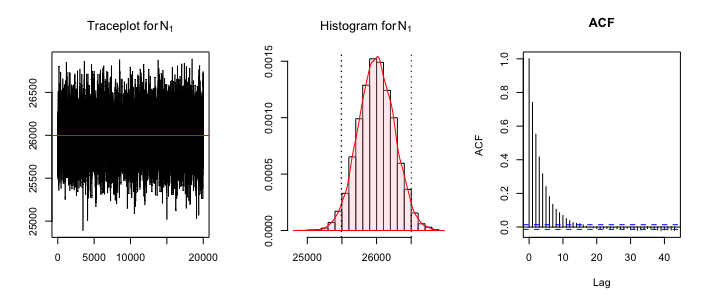
\includegraphics[scale=0.3]{N1_trace.png}
        \caption{Posterior samples for model 2 for the year 1968. Left: Trace, Middle: Histogram with 95\% credible intervals plotted vertically, Right: ACF for year 1968. For a better view and description see appendix. Just zoom it, man,}
    \label{traceN1}
\end{figure}
\begin{figure}[h!]
    \centering
    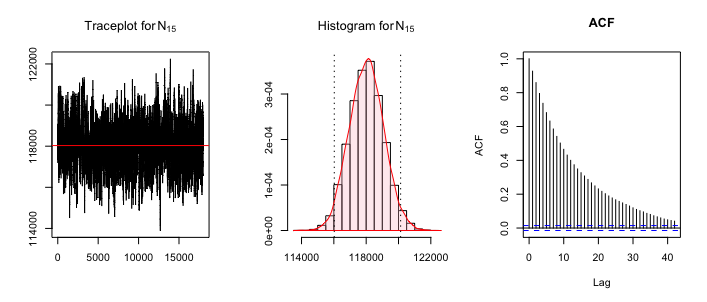
\includegraphics[scale=0.3]{N15.png}
    \caption{Trace and Histogram for population of Hawks at year 1982.}
    \label{traceN15}
\end{figure}
\begin{figure}[h!]
    \centering
    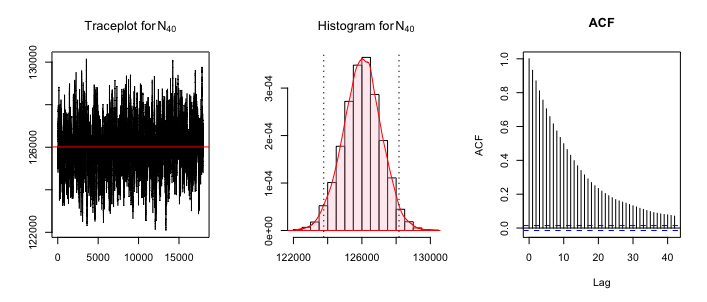
\includegraphics[scale=0.3]{N48.png}
    \caption{Trace and Histogram for population of Hawks at year 2015}
    \label{traceN48}
\end{figure}

Next we examine the posterior samples for $\theti$. These are summarized in table \ref{thsummary}. We see by the traceplots, histograms, and autocorrelation plots, that the conclusion is similar to $\Ni$ case.

\begin{table}[h!]
\centering
\begin{tabular}{rrrr}
  \hline
Year & Mean & 2.5\% & 97.5\% \\ 
  \hline
1981 & 0.0026 &0.0024& 0.0025 \\ 
  2004 & 0.0033 &0.0030& 0.0031 \\ 
  2012 & 0.0037 &0.0034 &0.0035\\ 
  2015 & 0.0036 & 0.0033 &0.0034 \\ 
   \hline
\end{tabular}
\caption{Summary of posterior samples of $\theti$}
\label{thsummary}
\end{table}

\begin{figure}[h!]
    \centering
    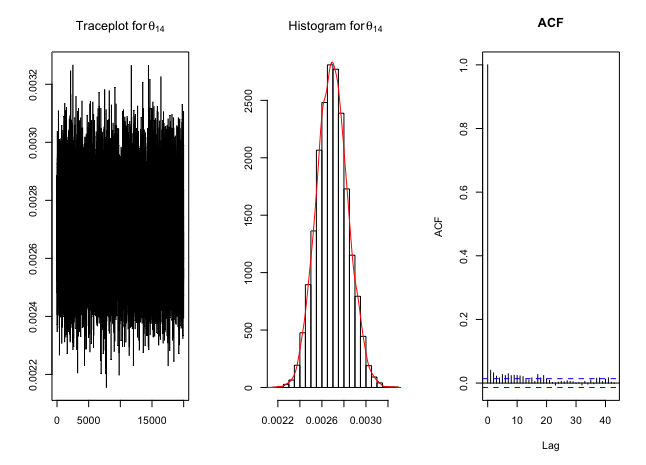
\includegraphics[scale = 0.35]{th14.png}
    \caption{Probability of observing a hawk at year 1981.}
    \label{th14}
\end{figure}

\begin{figure}[h!]
    \centering
    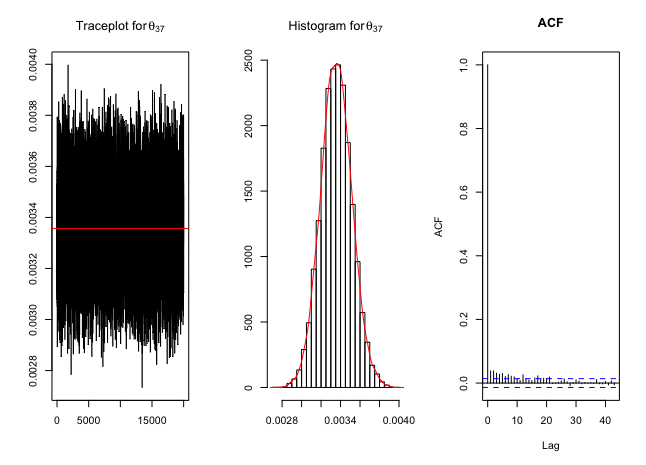
\includegraphics[scale = 0.35]{th37.png}
    \caption{Probability of observing a hawk at year 2004.}
    \label{th37}
\end{figure}

\begin{table}[h!]
\centering
\begin{tabular}{rrrr}
  \hline
Year & Mean & 2.5\% & 97.5\% \\ 
  \hline
1984 & 999.93 & 982.83 & 988.26 \\ 
  1988 & 999.64 & 982.84 & 988.10 \\ 
  1993 & 1000.32 & 982.75 & 988.67 \\ 
  1994 & 999.95 & 982.52 & 988.52 \\ 
   \hline
\end{tabular}
\caption{Summary of posterior samples of $\lami$ (these are chosen at random by the way, the same for $\theti$ and $\Ni$).}
\label{summary_lam}
\end{table}

Lastly, we examine the posterior samples for $\lami$. Summary is in Table \ref{summary_lam} and posterior traceplots, histograms and ACF plots for $\lami$ for randomly selected years are in figures \ref{lam17} and \ref{lam21}.
   


\begin{figure}[h!]
    \centering
    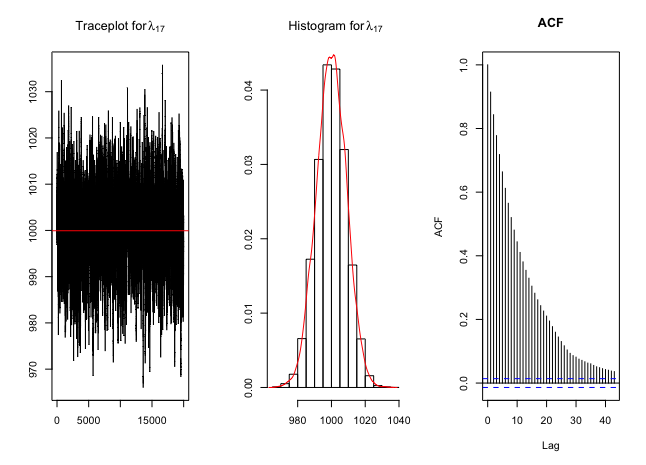
\includegraphics[scale = 0.35]{lam17.png}
    \caption{Posterior samples of $\lami$ for the year 1984.}
    \label{lam17}
\end{figure}

\begin{figure}[h!]
    \centering
    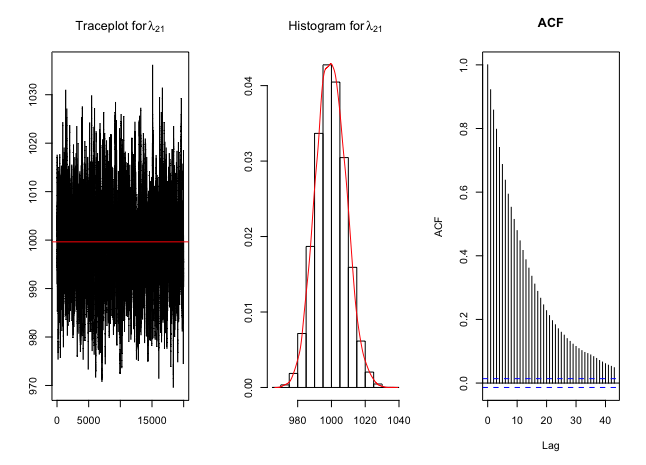
\includegraphics[scale = 0.35]{lam21.png}
    \caption{Posterior samples of $\lami$ for the year 1988.}
    \label{lam21}
\end{figure}

\clearpage
\section{Model Validation and Model Comparison}
First, we should explain the hierarchical structure of model 2 a bit more. The random variable $y_i\sim Bin(N_i,\theti)$ has a distribution given by

\begin{align}
    P(\Yequalsy) &= \sumyiO P(\Yequalsy, \Ni = \lcni)\\
    &= \sumyiO P(\Yequalsy|\Ni = \lcni)P(\Yequalsy) \\
    &= \sumyiNi \squarebk{\parenth{\lcni \choose \yi} \theti^{\yi} (1-\theti)^{\lcni - \yi} }\\
    &\tab \times \squarebk{\frac{\exp\curlies{-\lcni} (\lami\ci)^{\lcni}}{\lcni!}}\\
    &= \frac{(\lami\ci\theti)^\yi \exp\curlies{-\lami\ci}}{\lcni!}\\
    & \tab \sumyiNi \frac{((1-\theti)\lami\ci)^{\lcni-\yi}}{(\lcni - \yi)!}\\
    & =\frac{1}{\yi!}\parenth{(\lami\ci\theti)^{\yi} \exp\curlies{-\lami\ci\theti} }
\end{align}

Thus, for model 2, $y_i \sim \Pois(\lami \ci\theti)$ and any inference on $\yi$ is with respect to a $\Pois(\lami\ci\theti)$ distribution. Introducing $\Ni$ into the hierarchical model yields the following interpretation:  on average, $E\yi = \lami\ci\theti$ red hawks are observed.

To obtain posterior predictive replicates for Model 2, we simulate 200 Poisson random variables using our route count data, $\ci$, and posterior samples of $\theti, \lami$. The comparison of the actual Red Hawk sightings to the posterior  predictive  replicates, $y_i^{rep}$, show that this model does a good job at fitting the data (Figure \ref{M2_reps}).
Compared to our results using the prior specifications of model 1 (Figure \ref{M2_reps}), the difference is almost indistinguishable. Looking very, very closely there might be a slight improvement in predicting observations centered around the mean for model 2 (Figure \ref{compare}).

\begin{figure}[h!]
    \centering
    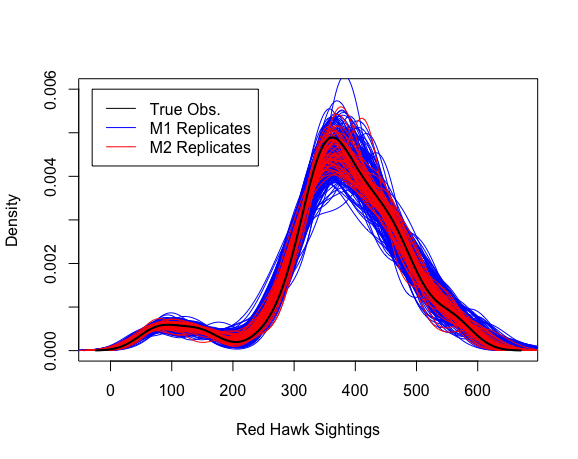
\includegraphics[scale=0.35]{comparison.png}
    \caption{200 samples from model 1 plotted against 200 samples from model 2. Here it is more obvious that model 2 \textit{may} provide posterior predictive samples that are closer to the true observations.}
    \label{compare}
\end{figure}

\begin{figure}[h!]
    \centering
    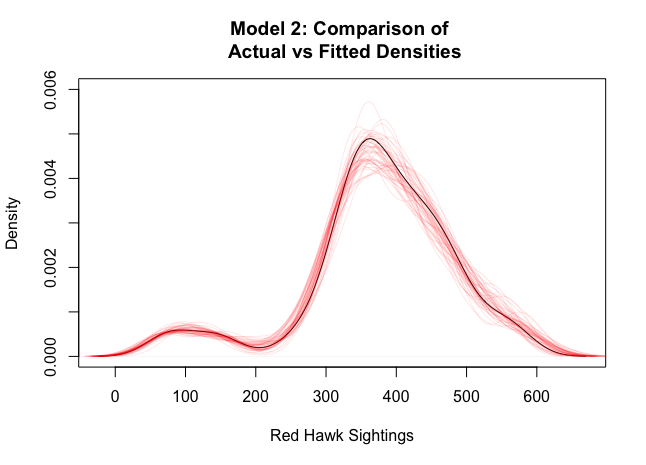
\includegraphics[scale=0.35]{FittedVReps.png}
    \caption{Distribution of the observed $y_i$ and the distributions of some of the posterior replicates ($y_i^{rep}$) for Model 2. Looking very, very closely there might be a slight improvement in predicting observations centered around the mean for model 2.}
    \label{M2_reps}
\end{figure}

\begin{figure}[h!]
    \centering
    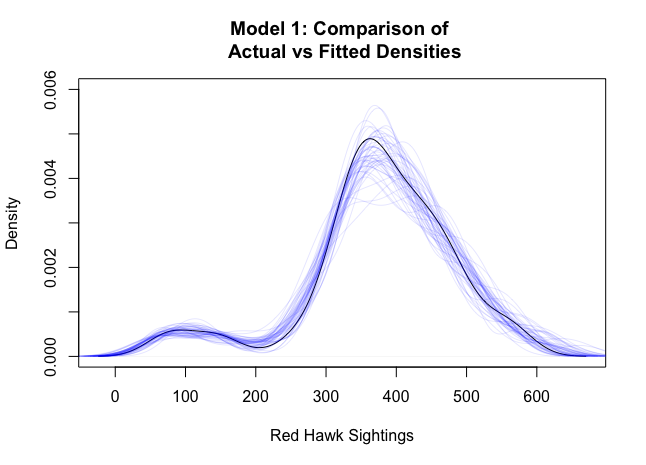
\includegraphics[scale=0.35]{m1_reps.png}
    \caption{Distribution of the observed $y_i$ and the distributions of some of the posterior replicates ($y_i^{rep}$) for Model 1.}
    \label{M1_reps}
\end{figure}


\begin{defn}[Gelfand \& Ghosh]
Let $\pmb{y}$ denote the observed data. Let $\mu_l = E(z_l|\pmb{y})$ and $\sigma^2_l = Var(z_l|\pmb{y})$. Then let $G = \sum_l (\mu_l - y_l)^2$, and $P = \sum_l \sigma^2_l$. The Gelfand and Ghosh criterion is defined as $D = G + P$, where $D$ seeks to reward goodness of fit penalizing complexity. So the smaller the D, the better the model.
\label{GG}
\end{defn}

Next, we use the Gelfand and Ghosh criterion to compare model 1 and model 2. For model 1, we get 1476.299 and for model 2 we get 1054.122. This value is smaller for model 2, which adds support to the earlier claim (Figure \ref{compare}) that model 2 better describes the data.

Intuitively, model 2 seems like it should be higher because it is more complex since more latent variables are involved and GG penalizes complex models. However, I showed in equations (1-7) that any marginal inference on $y_i$ is with respect to a Poisson($\lami\ci\theti$) distribution, with $\Ni$ playing no part at all. Thus, the complexity of model 2 is not much different than model 1. So the biggest factor contributing to the GG criterion is simply good-ness of fit. I am confident that I have defended my argument that model 2 is better than model 1.

\textbf{Estimate the probability of observing more than 450 red hawks in California in a yea with a route count of 120:}

Our model 2 (unlike my first attempt in exam 1) now includes the rate count. So what we are asked to predict is, given a completely new observation, for a new year with route count equal 120, what is the probability that the observed $\yi>450$. To calculate this, I use 200 posterior predicted replicates. From those replicates, I count how many are greater than 450 and and divide by the total replicates. This ratio comes out to be $0.2273$. Which is exactly what we discussed on exam 1.

\begin{figure*}[h!]
    \centering
    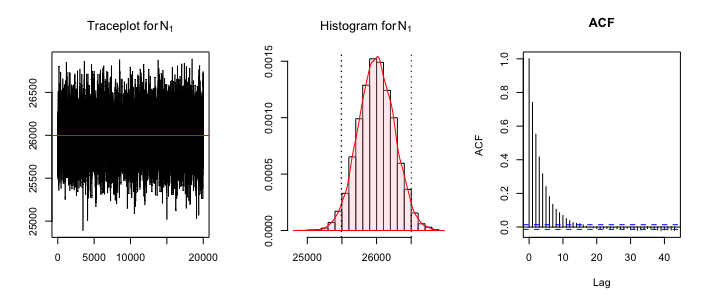
\includegraphics[scale=0.6]{N1_trace.png}
    \caption{Left:Trace, Middle: Histogram with 95\% credible intervals plotted vertically, Right: ACF for year 1968.}
    \label{append1}
\end{figure*}

\end{document}